\documentclass[11pt,onecolumn]{article}
\usepackage{amsmath,amssymb,graphicx,algorithmic,xspace,url}

\usepackage{listings,xcolor}
\lstset{ %
    language=Python,
    %backgroundcolor=\color{black!5},
    basicstyle=\footnotesize,
    showstringspaces=false,
    literate={``}{\textquotedblleft}1,
    deletestring=[b]",
    numbers=left,
    firstnumber=154,
    stepnumber=1,
    ,
}

\setlength{\pdfpagewidth}{8.5in}
\setlength{\pdfpageheight}{11in}
\setlength{\evensidemargin}{-0.1in} \setlength{\oddsidemargin}{-0.1in}
\setlength{\textwidth}{6.5in} \setlength{\textheight}{8.5in}
\setlength{\topmargin}{-0.25in}
%\setlength{\headheight}{0in}

%\setlength{\parindent}{0in}
%\setlength{\parskip}{0.125in}

\newcommand{\tuple}[1]{\ensuremath{\left\langle #1 \right\rangle}\xspace}
\newcommand{\set}[1]{\ensuremath{\left\{#1\right\}}\xspace}
\newcommand{\size}[1]{\ensuremath{\left|#1\right|}\xspace}
\newcommand{\true}{\ensuremath{\mathsf{true}}\xspace}
\newcommand{\false}{\ensuremath{\mathsf{false}}\xspace}
\let\originalleft\left
\let\originalright\right
\renewcommand{\left}{\mathopen{}\mathclose\bgroup\originalleft}
\renewcommand{\right}{\aftergroup\egroup\originalright}

\newtheorem{claim}{Claim}

\title{A reduction from min-edge to min-role}
\author{pg, mt}
\date{}
\sloppypar

\begin{document}
\maketitle

\noindent
We reduce the problem of finding an RBAC policy of the minimum number of edges, the ``min-edge'' problem, to that of finding an RBAC policy of the minimum number of roles, ``min-role''. The intent is to leverage techniques for min-role, to address instances of min-edge.

\vspace*{0.125in}
\noindent
Our reduction is really a ``chain'' of reductions:

\begin{quote}
	min-edge $\le$ Partial \textsc{Max-Sat} $\le$ Clique $\le$ Vertex Cover $\le$ Set Basis = min-role.
\end{quote}


\vspace*{0.125in}
\noindent
Two observations:
\begin{itemize}
\item In the last step, we exploit Vaidya et al.'s observation that min-role is exactly Set Basis. \url{https://doi.org/10.1145/1266840.1266870}
\item We seek to retain an optimization version in each reduction. That is, we recognize that min-edge is an optimization (minimization) problem. We do not want a reduction from it to, for example, CNF-SAT, because CNF-SAT is a ``purely'' decision problem only. If we exploited such a reduction, we would then have to employ, e.g., binary search, for the optimization objective --- this is something we do not like. Rather, we seek a reduction to an optimization problem.
\end{itemize}


\vspace*{0.125in}
\noindent
Now, onto the reductions.

\subsection*{min-edge $\le$ Partial \textsc{Max-Sat}}

\vspace*{0.125in}
\noindent
Partial \textsc{Max-Sat} is like \textsc{Cnf-Sat}, except that we partition the set of all clauses into two sets, $\tuple{\mathcal{H}, \mathcal{R}}$. The set of $\mathcal{H}$ are hard clauses --- these must be satisfied in a satisfying assignment. The set $\mathcal{R}$ comprises relaxable clauses --- we seek to either maximize or minimize the number of these clauses that are satisfied. We adopt the maximization version, given that Clique is a maximization problem. Denote this optimization (maximization) problem Max Partial \textsc{Max-Sat}.

\vspace*{0.125in}
\noindent
Thus, the first reduction we seek is from min-edge to Max Partial \textsc{Max-Sat}. We exploit the work from the Secrecy Resilience paper \url{https://doi.org/10.1145/3532105.3535030}.

\vspace*{0.125in}
\noindent
Specifically, we first adopt an upper-bound, denote it $n_r$, for the number of roles, and the boolean variables $c_{i,r}$ and $d_{j,r}$ for user $i$ assigned to role $r$, and role $r$ assigned to permission $j$, respectively. For the hard clauses $\mathcal{H}$, we adopt the clauses from under the first two bullets from the reduction in Section 3, ``New Reductions for Role and Edge Minimization in Role Mining'' in that paper. That is, we have the following two sets of clauses:
\begin{itemize}
\item For each user $i$ that possesses permission $j$ in the input UP matrix, we have the clauses $\left(c_{i,1}\wedge d_{j,1}\right) \vee \ldots \vee \left(c_{i,n_r} \wedge d_{j,n_r}\right)$. To convert to CNF, as proposed in that work, we first adopt the encoding as a circuit that is to the left of Figure 4 there, and then a reduction to clauses in CNF.
\item For each pair of user-permission where user $i$ does not possess permission $j$, we adopt the clauses $\left(\neg c_{i,1}\vee \neg d_{j,1}\right)\wedge\ldots\wedge\left(\neg c_{i,n_r}\vee \neg d_{j,n_r}\right)$.
\end{itemize}

\vspace*{0.125in}
\noindent
Those are the hard clauses, $\mathcal{H}$. For the relaxable clauses $\mathcal{R}$, we adopt $\neg c_{1,1}$, $\ldots$, $\neg c_{n_u, n_r}$, $\neg d_{1,1}$, $\ldots$, $\neg d_{n_p, n_r}$, where $n_u, n_p$ are the number of users and permissions respectively. We seek to maximize the number of these that are satisfied.

\subsection*{Partial \textsc{Max-Sat} $\le$ Clique}

\vspace*{0.125in}
\noindent
We adapt the reduction from CLRS for \textsc{Cnf-Sat} $\le$ Clique. \url{https://mitpress.mit.edu/9780262046305/introduction-to-algorithms/}. That reduction is said to be for 3-\textsc{Cnf-Sat} to Clique, but works, more generally, for \textsc{Cnf-Sat} to Clique. The reduction is as follows.

\vspace*{0.125in}
\noindent
Suppose the clauses in the \textsc{Cnf-Sat} instance are $c_1, \ldots, c_n$. And suppose the clause $c_i$ is $l_{i,1} \vee l_{i,2} \vee \ldots \vee l_{i,k}$, where each $l_{i,j}$ is a literal. For each literal in each clause, i.e., for each $l_{i,j}$ across all $i$ and $j$, we introduce a vertex, denote it $u_{i,j}$. We introduce an edge between vertices $u_{p,q}$ and $v_{r,s}$ if and only if:
\begin{itemize}
\item $u_{p,q}$ and $v_{r,s}$ are from different clauses, i.e., $p\not= r$. And,
\item The literals $l_{p,q}$ and $l_{r,s}$ to which the vertices $u_{p,q}$ and $v_{r,s}$ correspond, respectively, are consistent. That is, $l_{p,q} \not= \neg l_{r,s}$.
\end{itemize}

\vspace*{0.125in}
\noindent
Now, the instance of \textsc{Cnf-Sat} is satisfiable if and only if the graph has a clique of size $n$, the total number of clauses. This is because the literals that are set to $1$ in a satisfying assignment correspond exactly to the vertices in a clique.

\vspace*{0.125in}
\noindent
To adapt this reduction to Partial \textsc{Max-Sat}, we have to be a bit careful because we need to distinguish the hard and relaxable clauses. Simply treating the clauses in $\mathcal{H}$ and $\mathcal{R}$ as the same, i.e., the whole thing as an instance of \textsc{Cnf-Sat} does not work, as we have the second argument $k$, i.e., we require only $k$ of the clauses in $\mathcal{R}$ to be satisfied, and not all clauses in $\mathcal{H}\cup\mathcal{R}$.

\vspace*{0.125in}
\noindent
A next idea is to set the objective in the instance of Clique to $h + k$, where $\size{\mathcal{H}} = h$. This does not work either because it is possible that we have an assignment in which not all hard clauses are satisfied, yet $h+k$ total number of clauses are satisfied. E.g., suppose $\size{\mathcal{H}} = 1$, $\size{\mathcal{R}} = 2$ and $k = 1$. Then, $h+k = 2$, and we may have an assignment in which the (only) hard clause is not satisfied, but both relaxable clauses are satisfied.

\vspace*{0.125in}
\noindent
Here's an approach that appears to be correct. Let $r = \size{\mathcal{R}}$. For every clause $c\in\mathcal{H}$, we introduce $r + 1$ identical sets of vertices each corresponding to the clause $c$, but as though they are from different clauses in the reduction \textsc{Cnf-Sat} $\le$ Clique. Thus, if $h = \size{\mathcal{H}}$, we have $h\cdot r + h$ such sets of vertices (recall that we create one vertex per literal in a clause). For the clauses in $\mathcal{R}$ we introduce vertices just as we do for clauses in the \textsc{Cnf-Sat} $\le$ Clique reduction. Then, if the optimization objective in Partial \textsc{Max-Sat} is $k$, we set the optimization objective in Clique to $h\cdot r + h + k$.

\vspace*{0.125in}
\noindent
If the instance of Partial \textsc{Max-Sat} is true, it is pretty clear that the instance of Clique is true. For the other direction, suppose the instance of Partial \textsc{Max-Sat} is false. This can only be because one or both of the following is true for every assignment: (i) at least one clause in $\mathcal{H}$ is not satisfied, or, (ii) fewer than $k$ of the clauses in $\mathcal{R}$ are satisfied. In case (i), the maximum size of a clique is $(h-1)\cdot r + (h-1) + r = h\cdot r + h - 1 < h\cdot r + h + k$. In case (ii), the maximum size of a clique is $h\cdot r + h + k^\prime < h\cdot r + h + k$, given that $k^\prime < k$.

\subsection*{Clique $\le$ Vertex Cover}

\vspace*{0.125in}
\noindent
We adopt the straightforward reduction from CLRS. That reduction exploits the following claim. It leverages the notion of the complement of an undirected graph $G = \tuple{V, E}$. The complement of $G$, denoted $\overline{G}$ is the undirected graph $\tuple{V, \overline{E}}$, which has the same set of vertices as $G$, and:
\begin{align*}
	\tuple{u,v} \in E &\iff \tuple{u,v} \not\in \overline{E}
\end{align*}

\begin{claim}
$C$ is a clique in $G = \tuple{V,E}$ if and only if $V\setminus C$ is a vertex cover in $\overline{G}$.
\end{claim}

\vspace*{0.125in}
\noindent
Thus, towards a reduction, we would simply compute $\overline{G}$, and if the optimization objective in Clique is $k$, we set the optimization objective for Vertex Cover to $\size{V} - k$.

\vspace*{0.125in}
\noindent
\underline{\emph{Implementation note}}: We can directly reduce Partial \textsc{Max-Sat} $\le$ Vertex Cover using the above insights to save some implementation work, and perhaps time while running. We produce the vertices for the graph as we discuss above, and directly produce the edges $\overline{E}$ for the graph.

\subsection*{Vertex Cover $\le$ Set Basis}

\vspace*{0.125in}
\noindent
We adopt the reduction of Stockmeyer \url{https://dominoweb.draco.res.ibm.com/76642e18a923fcbf8525763c004aa783.html}. It works as follows.

\vspace*{0.125in}
\noindent
Assume our graph is $G = \tuple{V, E}$ where $E = \set{e_0, \ldots, e_{m-1}}$ such that for all $i$, $e_i = \tuple{e_{i,0}, e_{i,1}}$. In our output instance of min-role (i.e., UP bipartite graph), we introduce permissions as follows: (i) a permission for every vertex in $V$, and, (ii) two other permissions, denote than $a_i, b_i$ for every edge $e_i$. Thus, the total number of permissions is $\size{V} + 2m$.

\vspace*{0.125in}
\noindent
We introduce $3m$ users, denote them $u_0, \ldots, u_{3m-1}$. Every user has exactly three permissions, as follows.
\begin{itemize}
    \item User $u_0$ has permissions $a_0, e_{0,0}, e_{0,1}$. More generally, a user $u_{3i}$ for each $i = 0, \ldots, m-1$ has permissions $a_{i}, e_{i,0}, e_{i,1}$.
    \item User $u_1$ has permissions $a_0, e_{0,0}, b_0$. More generally, a user $u_{3i+1}$ for each $i = 0, \ldots, m-1$ has permissions $a_{i}, e_{i,0}, b_i$.
    \item User $u_2$ has permissions $a_0, e_{0,1}, b_0$. More generally, a user $u_{3i+2}$ for each $i = 0, \ldots, m-1$ has permissions $a_{i}, e_{i,1}, b_{i}$.
\end{itemize}

\vspace*{0.125in}
\noindent
That's it. Now the claim is that the graph has a vertex cover of size $k$ if and only if the output min-role instance has an RBAC policy of $k+2m$ roles.

\vspace*{0.125in}
\noindent
Consider the following example graph.

\vspace*{0.125in}
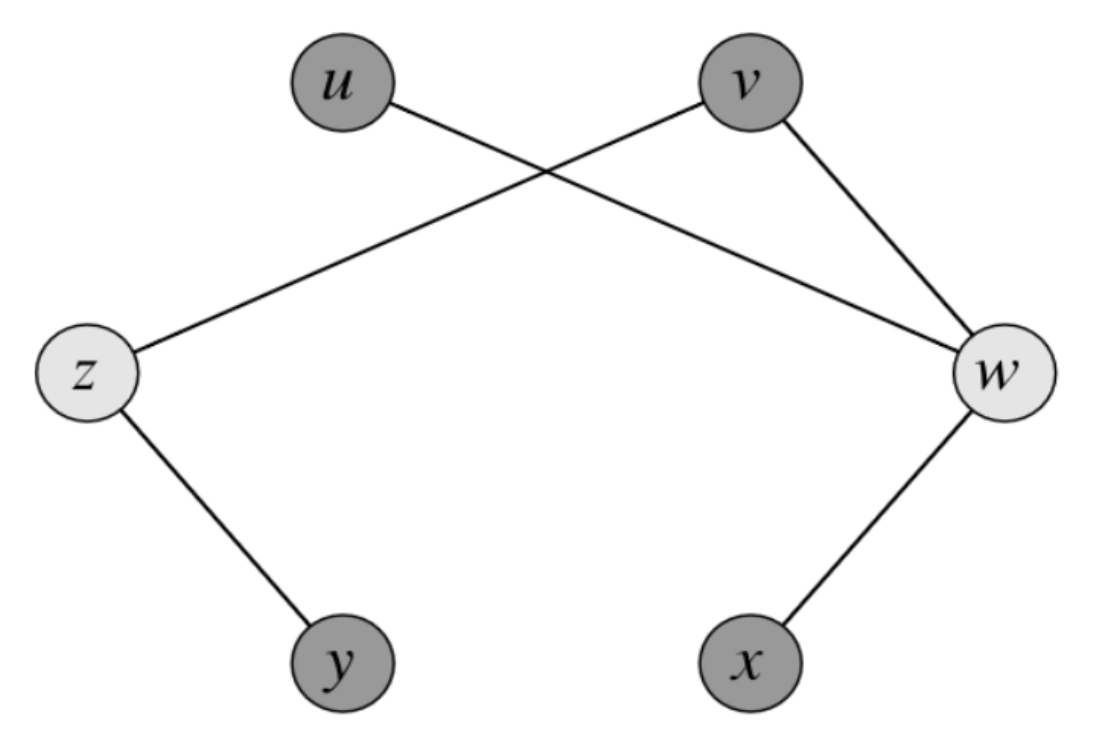
\includegraphics[width=0.33\linewidth]{examplegraph.png}

\vspace*{0.125in}
\noindent
Suppose $e_0 = \tuple{y,z}$, $e_1 = \tuple{z,v}$, $e_2 = \tuple{u,w}$, $e_3 = \tuple{v,w}$, and, $e_4 = \tuple{w,x}$. Then, we have the following as our output UP instance.

\vspace*{0.125in}
\begin{tabular}{l@{: }l@{\hspace*{0.25in}}l@{: }l@{\hspace*{0.25in}}l@{: }l@{\hspace*{0.25in}}l@{: }l@{\hspace*{0.25in}}l@{: }l}
$u_0$ & $a_0, y, z$ & $u_3$ & $a_1, z, v$ & $u_6$ & $a_2, u, w$ & $u_9$ & $a_3, v, w$ & $u_{12}$ & $a_4, w, x$\\
$u_1$ & $a_0, y, b_0$ & $u_4$ & $a_1, z, b_1$ & $u_7$ & $a_2, u, b_2$ & $u_{10}$ & $a_3, v, b_3$ & $u_{13}$ & $a_4, w, b_4$\\
$u_2$ & $a_0, z, b_0$ & $u_5$ & $a_1, v, b_1$ & $u_8$ & $a_2, w, b_2$ & $u_{11}$ & $a_3, w, b_3$ & $u_{14}$ & $a_4, x, b_4$
\end{tabular}

\vspace*{0.125in}
\noindent
For the above input, the minimum number of roles is $12$, which is what \textsf{maxsetsbp.py} reports. Thus, the minimum size for a vertex cover is $12 - 2m = 12 - 2\times 5 = 2$, which is correct.

\section*{Mapping the certificates}

\vspace*{0.125in}
\noindent
Once we have a certificate, i.e., solution, for min-role, we seek to map it to a solution for min-edge. This works in the natural way --- we first identify a vertex cover from the solution for min-role, and then the solution from min-edge from that vertex cover.

\vspace*{0.125in}
\noindent
For the first step, there will be roles in the solution to the min-roles instance such that each role is assigned exactly one permission that corresponds to a vertex. For the above example, following is the role-to-permissions map that \textsf{maxsetsbp.py} generates. The format is a role-number, following by a colon `:', followed by the set of permissions.

\begin{verbatim}
0: ['a0', 'y']
1: ['a0', 'b0']
2: ['a3', 'v']
3: ['a1', 'v']
4: ['w']
5: ['a2', 'b2']
6: ['a2', 'u']
7: ['a1', 'b1']
8: ['a4', 'b4']
9: ['z']
10: ['a3', 'b3']
11: ['a4', 'x']
\end{verbatim}

\vspace*{0.125in}
\noindent
As we can see, we have exactly two roles, roles $4$ and $9$, each of which has exactly one permission assigned, which is a vertex from the graph. This yields exactly a solution to the vertex cover instance; in this example, a vertex cover of minimum size for the graph is exactly $\set{w, z}$.

\vspace*{0.125in}
\noindent
For the second step, i.e., to find the solution to min-edge given a vertex cover, we first identify the $c_{i,r}$ and $d_{j,r}$ that are set to true. Recall that in the Partial \textsc{Max-Sat} $\le$ Vertex Cover reduction, the vertex cover corresponds exactly to those clauses. That is, the relaxable clauses that are part of the solution to the Clique instance are those $\neg c_{i,r}$ and $\neg d_{j,r}$ that are true. Therefore, the $\neg c_{i,r}$ and $\neg d_{j,r}$ that are false for Clique are exactly the Vertex Cover. That is, those $c_{i,r}$ and $d_{j,r}$ that are the $\neg c_{i,r}$ and $\neg d_{j,r}$ vertices in a solution to the Vertex Cover instance are exactly the edges in the min-edge RBAC policy.

\vspace*{0.125in}
\noindent
Given the $c_{i,r}$ and $d_{j,r}$ that are edges in a min-edge RBAC policy, we can generate the role-to-user and role-to-permission map in a straightforward way. The following lines of code from \textsf{minedgetoilp.py} show how:

\hspace*{0.5in}
\begin{minipage}{0.95\linewidth}
\begin{lstlisting}
    roletousersmap = dict()
    roletopermsmap = dict()

    for r in range(nr):
        for u in up:
            v = m.getVarByName('c_'+str(u)+'_'+str(r))
            if v.getAttr(GRB.Attr.X):
                if r not in roletousersmap:
                    roletousersmap[r] = set()
                (roletousersmap[r]).add(u)
        for p in pu:
            v = m.getVarByName('d_'+str(p)+'_'+str(r))
            if v.getAttr(GRB.Attr.X):
                if r not in roletopermsmap:
                    roletopermsmap[r] = set()
                (roletopermsmap[r]).add(p)
\end{lstlisting}
\end{minipage}

\section*{Efficiency}

\vspace*{0.125in}
\noindent
The entire reduction is $\Theta(n^4)$ in the worst-case, starting with an input to min-edge of size $n$. The min-edge $\le$ Partial \textsc{Max-Sat} reduction is $\Theta(n^2)$ in the worst-case. And the Partial \textsc{Max-Sat} $\le$ Vertex Cover reduction is also $\Theta(n^2)$ in the worst-case. Also, there is a $3\times$ blowup in the Vertex Cover $\le$ min-role reduction.

\vspace*{0.125in}
\noindent
The largest benchmarks have size approximately $1 MB$ on disk. This may render this reduction impractical for the largest benchmark inputs\ldots but we'll need to try it, because we may not hit the worst-case of $\Theta(n^4)$.


\end{document}

